\documentclass[12pt]{article}

\usepackage{sbc-template}

\usepackage{graphicx,url}
%\usepackage[brazil]{babel}   
\usepackage[utf8]{inputenc}
\usepackage{float}
\usepackage{listings}
\usepackage{xcolor} % para cores
\usepackage{subcaption}


     
\sloppy

\title{MO446/MC949 - Visão Computacional\\Reconstrução 3D}

\author{Caio R. Teixeira , Flávio A. P. Cunha , Isac L. S. Braga \\ Paula M. da Fonseca, Vítor de M. Calhau}


\address{Universidade Estadual de Campinas
  (UNICAMP)\\
  Campinas -- SP -- Brazil\\
  Instituto de Computação
  \email{\{c212661,f197083,i260514,p138995,v248740\}@dac.unicamp.br}
}

\begin{document} 

\maketitle


\section{Coleta das Imagens e Preparação}
Afim de assegurar uma base sólida para a reconstrução tridimensional, a etapa de captura de imagens foi conduzida por meio de uma abordagem sistemática e criteriosa. Foram realizadas cinco sessões fotográficas consecutivas, cada uma delas gerando um lote de aproximadamente 47 imagens, o que totalizou um acervo significativo para o processamento fotogramétrico. A opção por repetir o processo em múltiplas etapas permitiu não apenas garantir a sobreposição desejada entre 60\% e 80\%, mas também explorar uma variabilidade angular e de altura mais consistente, enriquecendo a representação visual do objeto em seus múltiplos aspectos.

O equipamento utilizado foi um iPhone 11, cujo sensor e lente foram aproveitados sob condições controladas de iluminação difusa, em ambiente interno. Um dos elementos centrais do setup foi a criação de um “fundo infinito” improvisado, utilizando uma camiseta de tonalidade preta. Essa solução, ainda que prática, demandou um cuidado meticuloso durante o enquadramento, uma vez que qualquer desvio no posicionamento da câmera poderia comprometer a homogeneidade do pano de fundo e, consequentemente, a eficácia do seu papel no realce do objeto.

A exposição e o foco foram ajustados manualmente e mantidos fixos ao longo de todas as sessões, assegurando coerência lumínica e evitando flutuações indesejadas que poderiam interferir no alinhamento das imagens. A realização de diversas tomadas em sequência revelou-se uma estratégia fundamental para corrigir imperfeições eventuais, ajustar pequenos desvios de enquadramento e ampliar a diversidade de pontos de vista, consolidando um conjunto de dados mais robusto e confiável para as etapas subsequentes de processamento no pipeline de reconstrução 3D.

\section{Detecção e Extração de Características}

Os descritores de características tem o objetivo de extrair informações distintivas de keypoints em imagens, permitindo a identificação e correspondência de características entre diferentes pontos de visão.
Para este trabalho, foram testados 2 descritores diferentes, SIFT e AKAZE.

O SIFT utiliza características de ponto flutuante de 128 dimensões, sendo invariante a rotação, escala e parcialmente iluminação. Sua principal vantagem seria a alta qualidade das correspondências e robustez a variações ambientais, mas com alto custo computacional e possível lentidão.

O AKAZE, por outro lado, utiliza descritores binários, resultando em operações de matching mais rápidas através da utilização de distância de Hamming. No entanto, apresenta menor robustez a mudanças de iluminação e maior sensibilidade a ruído, algo que ficou bem evidente em nossos testes iniciais para escolha do descritor.

Para tentar otimizar o AKAZE, implementamos várias estratégias: aumento do threshold de detecção para 0.001, redução do número de octaves e layers, aplicação de filtros por tamanho (removendo keypoints menores que 5 pixels), filtros por resposta (mantendo apenas os 20\% mais fortes), e limitação máxima de 1000 keypoints por imagem.

\begin{figure}[H]
    \centering
    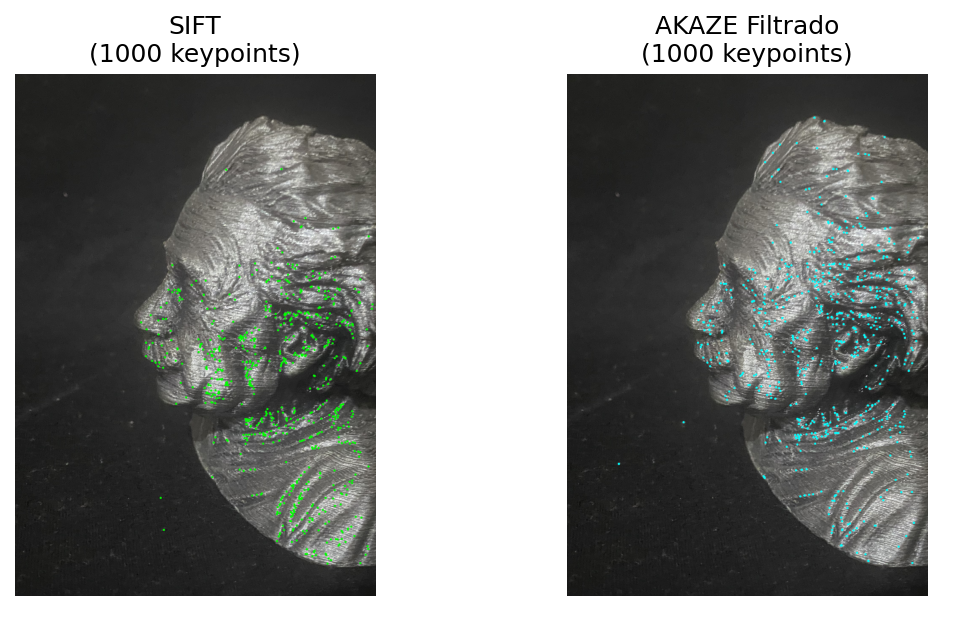
\includegraphics[width=0.5\textwidth]{images/akaze_sift_comparison_5.png}
    \caption{Comparação dos keypoints dos descritores SIFT vs AKAZE.}
    \label{fig:sift}
\end{figure}

Essas otimizações reduziram os ruídos e melhoraram a qualidade das correspondências.
No entanto, mesmo com tais otimizações, decidimos permanecer com o SIFT, já que em nos testes realizados, ele apresentou maior robustez e ofereceu maior confiabilidade na estimação de poses de câmera e triangulação de pontos 3D, resultando em reconstruções mais precisas e estáveis. A robustez do SIFT a mudanças de iluminação e textura é particularmente valiosa no contexto do projeto, considerando que as condições de captura tiveram variações.

Um outro ponto a favor do SIFT é usa utilização por padrão no biblioteca de SfM chamada COLMAP, que utilizamos para montar o pipeline de reconstrução completo nas próximas etapas.

\section{Emparelhamento e Geometria Epipolar}
Na etapa de emparelhamento de características  é realizado o alinhamento correto das regiões correspondentes. Para comparar os descritores, foi utilizada a abordagem FLANN (Fast Library for Approximate Nearest Neighbors), padrão no pipeline do COLMAP. Diferente do método \textit{brute force}, que realiza uma busca exaustiva, o FLANN encontra correspondências de forma aproximada e otimizada, oferecendo a performance necessária para processar eficientemente um grande volume de características.

Após o emparelhamento inicial, o conjunto de correspondências candidatas frequentemente contém outliers (pares falsos) que precisam ser filtrados. O Ratio Test de Lowe é um filtro heurístico fundamental para essa tarefa, cuja lógica se baseia em avaliar a distintividade de uma correspondência.
Ele funciona verificando se a melhor correspondência para um ponto é significativamente superior à segunda melhor. Se não for, o par é considerado incerto e removido, garantindo que apenas as correspondências mais confiáveis e únicas prossigam para a próxima etapa.

Para visualização das correspondências, foi utilizada a ferramenta de visualização do próprio COLMAP, que mostra os pares de imagens com o maior número de correspondências (usualmente, as com maior sobreposição) e desenha as linhas de conexão, como é possível observar na Figura \ref{fig:matches}.

\begin{figure}[h!]
\centering
\includegraphics[width=0.8\textwidth]{images/matches_comparison.png}
\caption{Imagens comparando as correspondências entre pares de duas imagens: a) alta sobreposição (1 e 2), b) pouca sobreposição (2 e 14), c) alta sobreposição (14 e 16)}
\label{fig:matches}
\end{figure}

Após a correspondência entre imagens, é gerado um \textit{grafo de cena}, no qual os nós representam as imagens e as arestas representam pares geometricamente verificados. Tal verificação geométrica é realizada por meio da estimação de modelos epipolares (matriz fundamental ou essencial), com robustez assegurada pela técnica RANSAC. O resultado desta validação é um conjunto de correspondências inliers (pares corretos) e a estimativa do movimento relativo (rotação e translação) entre as câmeras.

\section{Reconstrução 3D e geração da nuvem de pontos}

Com base no grafo gerado na etapa anterior, procede-se à \textbf{inicialização da reconstrução}, que parte de um par inicial de imagens escolhido de modo a maximizar a sobreposição e minimizar a ambiguidade geométrica. A partir deste par, obtém-se uma reconstrução inicial em escala relativa, que fornece as primeiras poses de câmera. Na etapa de \textbf{registro incremental}, novas imagens são incorporadas ao modelo por meio da resolução do problema \textit{Perspective-n-Point} (PnP), utilizando correspondências 2D–3D entre pontos já triangulados e suas projeções na nova imagem. Dessa forma, expande-se o conjunto de poses de câmera estimadas. Em paralelo, procede-se à \textbf{triangulação}, pela qual novos pontos tridimensionais são adicionados à nuvem esparsa a partir de múltiplas observações, aumentando a robustez e a completude do modelo.

Devido à natureza incremental do processo, incertezas nas poses das câmeras e nos pontos triangulados tendem a se acumular. Para mitigar tais erros, geralmente emprega-se o \textbf{Bundle Adjustment} (BA), que consiste em um refinamento não linear conjunto dos parâmetros de câmera e da estrutura 3D, minimizando o erro de reprojeção global. O BA é aplicado iterativamente, tanto de forma local quanto global, assegurando consistência e precisão ao modelo. 

Ao final da execução do pipeline, são produzidos dois resultados fundamentais: (i) uma \textbf{nuvem de pontos esparsa}, que representa a estrutura tridimensional básica da cena; e (ii) as \textbf{poses de câmera} (parâmetros extrínsecos de translação e rotação) associadas a cada imagem registrada. Esses resultados constituem a base para a geração de malhas, e podemos vê-los na Figura \ref{fig:sparsePoint3}.

\begin{figure}[H]
    \centering
    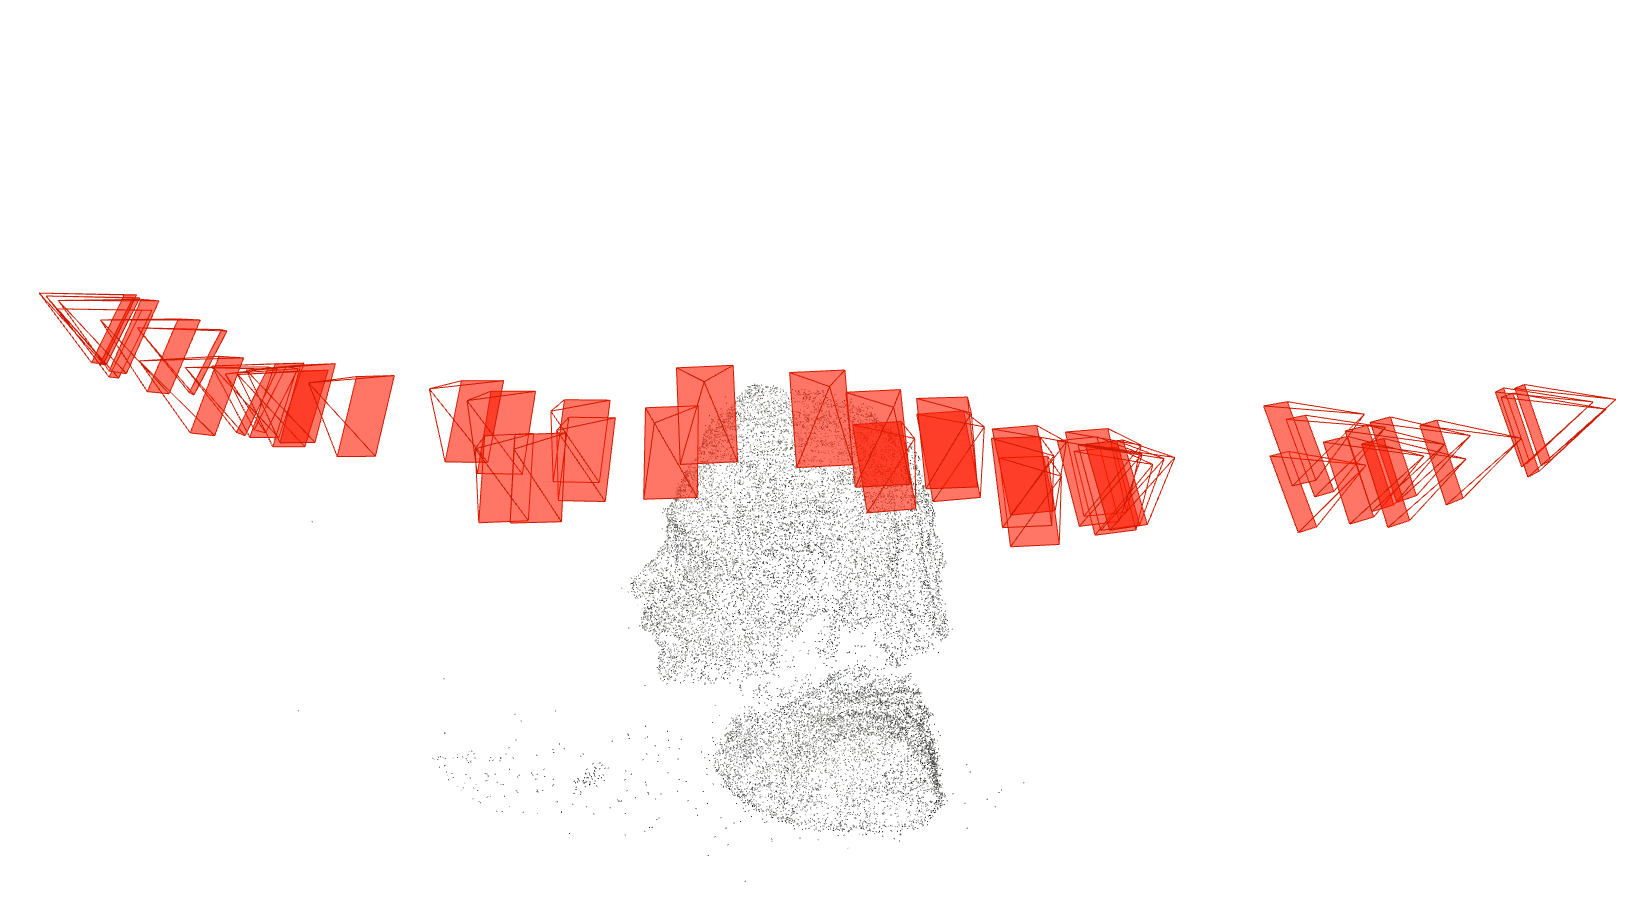
\includegraphics[width=.5\textwidth]{images/view_sparsePoint3.png}
    \caption{Nuvem esparsa de pontos e poses de câmera}
    \label{fig:sparsePoint3}
\end{figure}

Conforme evidenciado por \cite{schoenberger2016sfm}, a combinação de verificações geométricas robustas, estratégias de seleção da próxima melhor vista, triangulação eficiente e refinamentos iterativos via BA contribui para ganhos substanciais em robustez, precisão e completude, mesmo em cenários de grande escala e com coleções de imagens não estruturadas.

\subsection{Geração da malha no MeshLab}

Após a obtenção da nuvem de pontos esparsa por meio da reconstrução via SfM, procedeu-se à geração da malha tridimensional utilizando o software MeshLab. O processo foi conduzido em três etapas principais, cada uma delas aplicada com o intuito de refinar a qualidade geométrica da malha e assegurar maior realismo na representação da cena.

No primeiro estágio, empregou-se o filtro \textit{Compute Normals for Point Sets}. Esse procedimento calcula as normais locais da nuvem de pontos, fundamentais para a reconstrução da superfície, uma vez que fornecem a orientação necessária para os algoritmos de malhagem. O cálculo adequado das normais é essencial para evitar artefatos e inconsistências durante a etapa subsequente de reconstrução.

Em seguida, aplicou-se o filtro \textit{Surface Reconstruction: Screened Poisson}. O método de reconstrução por Poisson, na sua variante \textit{Screened}, é amplamente utilizado por sua robustez frente a ruídos e por permitir a recuperação de superfícies contínuas e suaves a partir da nuvem de pontos com normais associadas. Esse procedimento gera a malha inicial, interpolando de forma consistente a estrutura geométrica implícita nos dados.

Por fim, para refinar a qualidade superficial da malha gerada, utilizou-se o filtro \textit{Laplacian Smooth}. O método de suavização Laplaciana tem como objetivo reduzir irregularidades locais e eliminar ruídos residuais, garantindo uma superfície mais uniforme e esteticamente adequada. Importante ressaltar que a suavização foi aplicada de modo controlado, de forma a preservar as principais características geométricas do modelo sem comprometer sua fidelidade estrutural. A aplicação sequencial dessas etapas resultou em uma malha tridimensional consistente como pode ser visto na Figura \ref{fig:model}.

\begin{figure}[H]
    \centering
    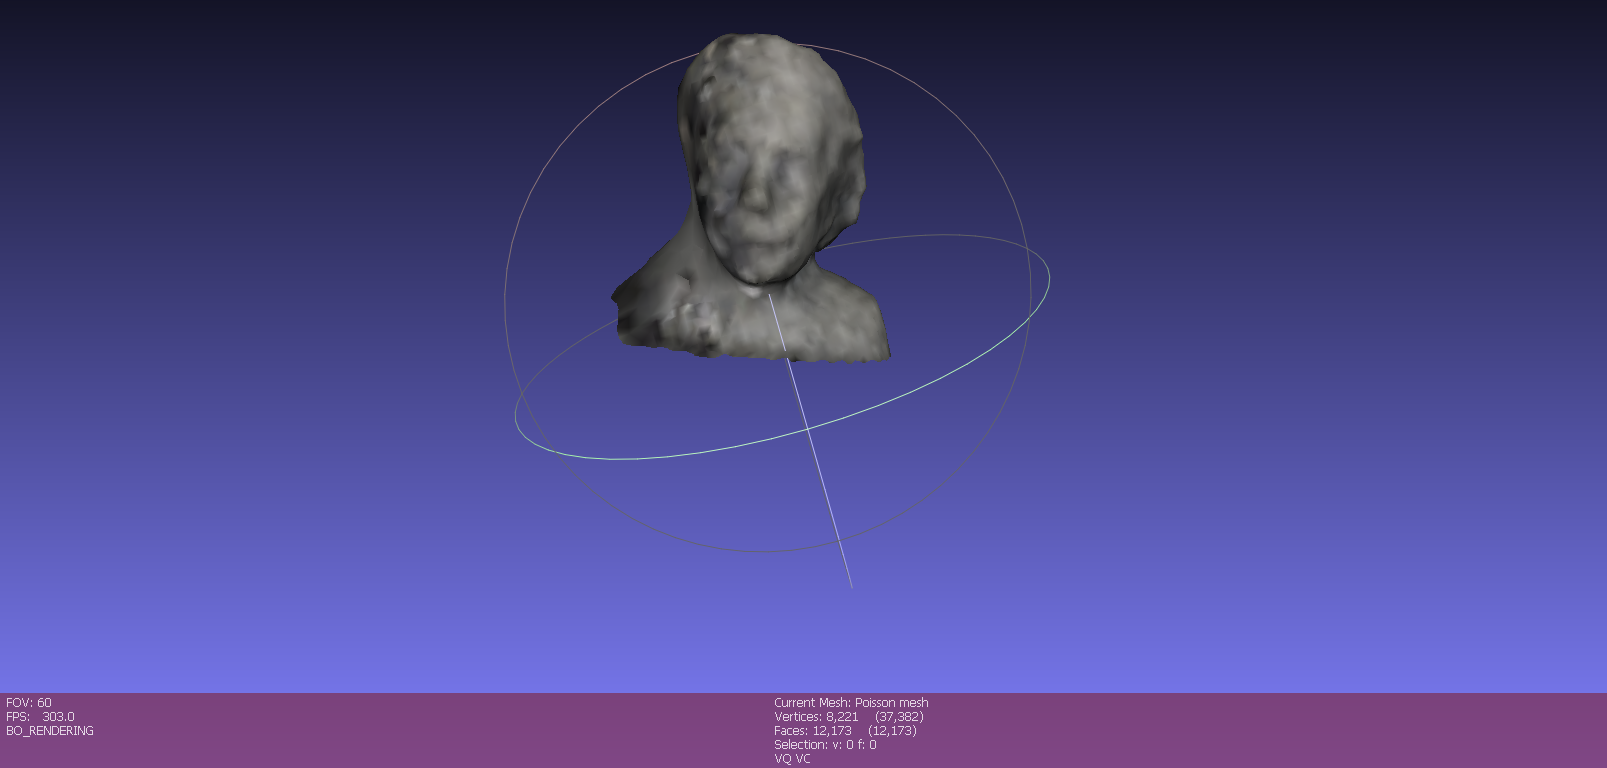
\includegraphics[width=.5\textwidth]{images/modelo_3d.png}
    \caption{Visualização do modelo 3D no meshlab}
    \label{fig:model}
\end{figure}

\subsection{Extra: Recuperação da escala absoluta }

A reconstrução obtida por meio de técnicas de \textit{Structure-from-Motion} apresenta, em sua forma inicial, uma escala arbitrária, uma vez que a metodologia baseia-se exclusivamente em informações relativas derivadas da geometria epipolar. Para possibilitar análises métricas e garantir a comparabilidade com dimensões reais, tornou-se necessário o procedimento de recuperação da escala absoluta do modelo. Esse processo foi realizado em duas etapas principais: medição de referência e aplicação do fator de escala.

A primeira etapa consistiu no uso da ferramenta \textit{Measuring Tape Tool}, disponível no MeshLab. Para tal, selecionou-se o ícone da ferramenta na barra de ferramentas e, em seguida, efetuou-se um clique em dois pontos distintos do modelo tridimensional, definindo assim um segmento de medição. O software exibiu a distância calculada entre esses pontos, permitindo que o valor fosse registrado como o comprimento medido no modelo como pode ser visto na imagem abaixo.

De posse da medida de referência, calculou-se o \textbf{fator de escala} como a razão entre o comprimento real do objeto e o comprimento correspondente medido no modelo tridimensional. Esse fator constitui a proporção necessária para alinhar a escala arbitrária do modelo com a escala real. Para aplicar tal ajuste no MeshLab, utilizou-se o filtro \textit{ Transform: Scale}, no qual o valor calculado do fator de escala foi inserido. Dessa forma, a malha reconstruída passou a refletir as dimensões métricas reais como pode ser visto na Figura \ref{fig:model_scale}.

\begin{figure}[H]
    \centering
    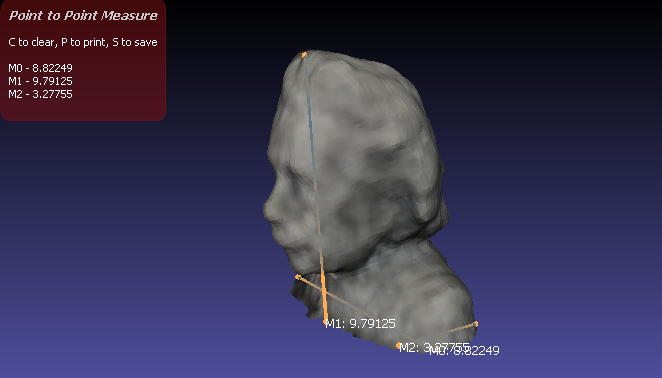
\includegraphics[width=.5\textwidth]{images/measures_model3D_scale.png}
    \caption{Medidas do modelo 3D no meshlab após aplicar o fator de escala}
    \label{fig:model_scale}
\end{figure}


\section{Avaliação e Ablative Study}
Para avaliar a qualidade do nosso modelo de forma numérica, independendo da observação direta do resultado final, podemos analisar as seguintes métricas:\\
- \textbf{Erro de reprojeção}: É obtido a partir da reprojeção dos pontos do modelo 3D em pixeis nos referênciais originais das imagens, após isso é medida a diferença entre a posição original do pixel, e a posição do pixel reconstruído. Um valor de erro baixo para essa métrica representa uma boa consistência geométrica no modelo obtido.\\
- \textbf{Número de pontos}: representa a quantidade de pontos reconstruídos na nuvem esparsa ou densa. Um número maior para essa métrica pode indicar a obtenção mais detalhes no modelo. Embora possa depender bastante da complexidade do objeto, pode ser usado como uma métrica de detalhamento e completude do modelo.\\
Com o conjunto dessas métrica, podemos obter uma avaliação mais completa do modelo, sendo possível analisar a cobertura e detalhamente pela métrica  de número de pontos, e garantindo uma consistência geométrica que faz sentido a partir do erro de reprojeção.

Ao tomar essas métricas para nosso resultado final da nuvem esparsa, observamos:\\
\textbf{Erro de Reprojeção Médio:} 1.05338\\
\textbf{Quantidade de Pontos:} 15268\\
\textbf{Densidade (pontos/unidade³):} 106.1\\
E ao realizar as medidas na malha do objeto final:
\textbf{Quantidade de pontos}: 6159\\
\textbf{Densidade aproximada (pontos / unidade de área)}: 28.43686411464795\\

Combinando os resultados obtidos temos um indicativo que a reconstrução foi satisfatória, da do que o erro médio da nuvem esparsa foi de aproximadamente 1,05 pixels, de forma que o pixel reprojetado geralmente está na vizinhança do original, levando a uma boa consistência geométrica. Além disso, na quantidade de pontos, apesar de não haver um referêncial global de um número desejado, ao observar o resultado, é possível concluir que os 15 mil pontos obtidos dão uma cobertura boa da imagem, com exceção de um dos lados, no para o qual poucas imagens foram capturadas. já para a malha final obtida, temos uma quantidade menor de pontos, o que é explicado pelo uso dos algoritmos Screened Poisson e do filtro Laplacian Smooth, que suavizam a superfície final, removendo pontos irregulares ou redundantes.

Para o Ablative Study, variamos o threshold de erro máximo do ransac, que tem relação com o erro de reprojeção. No entanto, como já obtivemos um erro médio baixo para o threshold padrão (4.0 pixels), o aumento ou diminuição dele afetou pouco as métricas de quantidade de pontos e erro médio. No entanto foi possível notar o tradeoff, no qual com a diminuição do threshold temos uma diminuição tanto na quantidade de pontos quanto no erro médio, resultando um uma consistência geométrica melhor, mas diminuindo pontos, o que pode gerar buracos, diminuir detalhamento, ou diminuir a cobertura do objeto final.




\bibliographystyle{sbc}
\bibliography{sbc-template}

\end{document}
